\documentclass[a4paper,10pt]{article}
\usepackage{fullpage}
\usepackage[british]{babel}
\usepackage[T1]{fontenc}
\usepackage{amsmath}
\usepackage{amssymb}
\usepackage[T1]{fontenc}
\usepackage{natbib}
\usepackage[utf8]{inputenc}
%\usepackage{amsthm} \newtheorem{theorem}{Theorem}
\usepackage{color}
\usepackage{float}
\usepackage{authblk}
\usepackage{todonotes}
\usepackage{algorithmicx}
\usepackage{algpseudocode}% http://ctan.org/pkg/algorithmicx

\usepackage{caption}
\DeclareCaptionFont{white}{\color{white}}
\DeclareCaptionFormat{listing}{\colorbox{gray}{\parbox{\textwidth}{#1#2#3}}}
\captionsetup[lstlisting]{format=listing,labelfont=white,textfont=white}

\usepackage{alltt}
\usepackage{listings}
\usepackage{algorithm}
%\usepackage{algorithmicx}
\usepackage{subfig}
\lstset{% parameters for all code listings
language=Python,
frame=single,
basicstyle=\small, % nothing smaller than \footnotesize, please
tabsize=2,
numbers=left,
% framexleftmargin=2em, % extend frame to include line numbers
%xrightmargin=2em, % extra space to fit 79 characters
breaklines=true,
breakatwhitespace=true,
prebreak={/},
captionpos=b,
columns=fullflexible,
escapeinside={\#*}{\^^M}
}



\usepackage{tikz}
\usetikzlibrary{arrows}
\usetikzlibrary{automata,positioning}

\newcommand{\abpsender}[1][]{

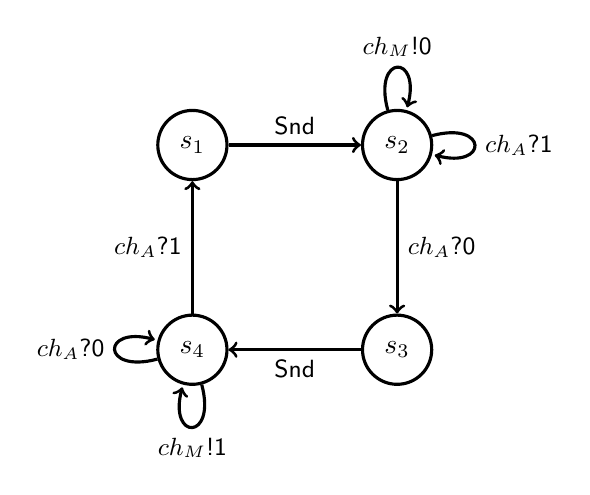
\begin{tikzpicture} [->,auto,node distance=2.6cm,line width=0.4mm]
  \node[state] (1) {$s_1$};
  \node[state] (2) [right of=1] {$s_2$};
  \node[state] (3) [below of=2] {$s_3$};
  \node[state] (4) [left of=3] {$s_4$};

  \path[every node/.style={font=\sffamily\small}]
    (1) edge node [above] {Snd} (2)
    (2) edge node [right] {$ch_A$?0} (3)
        edge [loop right] node {$ch_A$?1} (2)
        edge [loop above] node {$ch_M$!0} (2)
    (3) edge node [below] {Snd} (4)
    (4) edge node [left] {$ch_A$?1} (1)
        edge [loop left] node {$ch_A$?0} (4)
        edge [loop below] node {$ch_M$!1} (4);
\end{tikzpicture}
}

\newcommand{\abpreceiver}[1][]{
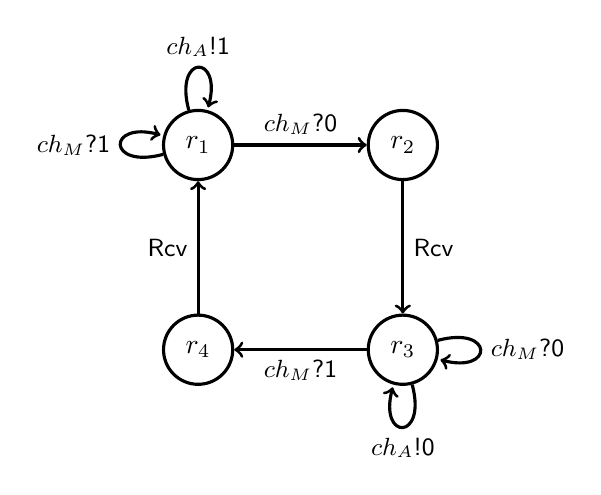
\begin{tikzpicture} [->,auto,node distance=2.6cm,line width=0.4mm]

  \node[state] (1) {$r_1$};
  \node[state] (2) [right of=1] {$r_2$};
  \node[state] (3) [below of=2] {$r_3$};
  \node[state] (4) [left of=3] {$r_4$};

  \path[every node/.style={font=\sffamily\small}]
    (1) edge node [above] {$ch_M$?0} (2)
        edge [loop left] node {$ch_M$?1} (1)
        edge [loop above] node {$ch_A$!1} (1)
    (2) edge node [right] {Rcv} (3)
    (3) edge node [below] {$ch_M$?1} (4)
        edge [loop right] node {$ch_M$?0} (3)
        edge [loop below] node {$ch_A$!0} (3)
    (4) edge node [left] {Rcv} (1);

\end{tikzpicture}
}


\newcommand{\swsender}[1][]{
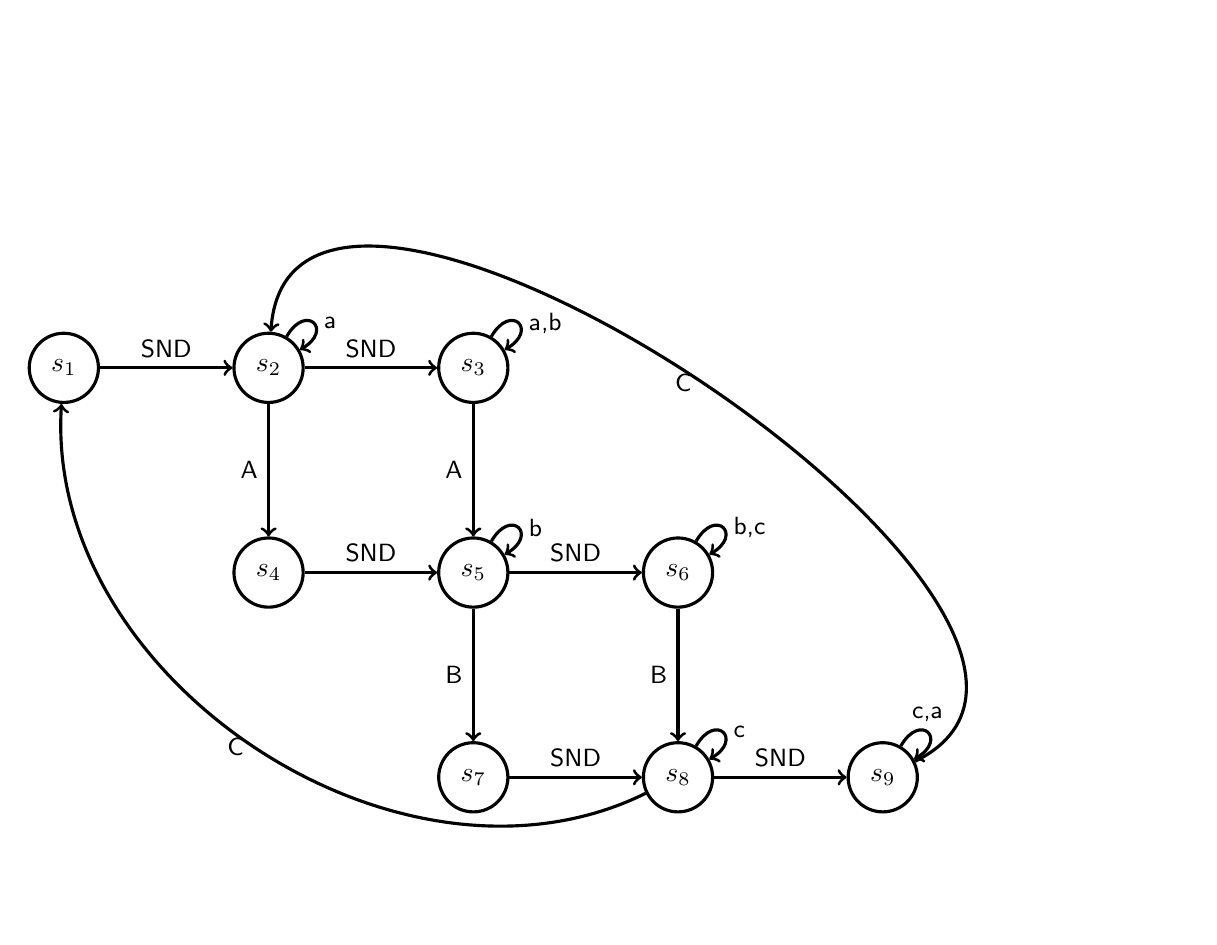
\begin{tikzpicture} [->,auto,node distance=2.6cm,line width=0.4mm]
  \node[state] (1) {$s_1$};
  \node[state] (2) [right of=1] {$s_2$};
  \node[state] (3) [right of=2] {$s_3$};
  \node[state] (4) [below of=2] {$s_4$};
  \node[state] (5) [below of=3] {$s_5$};
  \node[state] (6) [right of=5] {$s_6$};
  \node[state] (7) [below of=5] {$s_7$};
  \node[state] (8) [below of=6] {$s_8$};
  \node[state] (9) [right of=8] {$s_9$};

  \path[->,every loop/.style={in=30, out=60, looseness=3}, every node/.style={font=\sffamily\small}]
    (1) edge node [above] {SND} (2)
    (2) edge node [above] {SND} (3)
        edge [loop right] node {a} (2)
        edge node [left] {A} (4)
    (3) edge node [left] {A} (5)
        edge [loop right] node {a,b} (3)
    (4) edge node [above] {SND} (5)
    (5) edge node [above] {SND} (6)
        edge [loop right] node {b} (5)
        edge node [left] {B} (7)
    (6) edge node [left] {B} (8)
        edge [loop right] node {b,c} (6)
    (7) edge node [above] {SND} (8)
    (8) edge node [above] {SND} (9)
        edge [loop right] node {c} (8)
        edge [bend left=60] node [left] {C} (1)
    (9) edge [bend right=120] node [left] {C} (2)
        edge [loop above] node {c,a} (9);




\end{tikzpicture}
}

\newcommand{\swreceiver}[1][]{
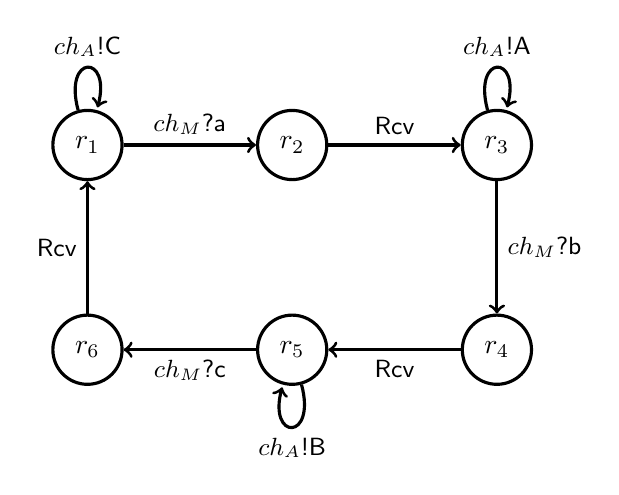
\begin{tikzpicture} [->,auto,node distance=2.6cm,line width=0.4mm]

  \node[state] (1) {$r_1$};
  \node[state] (2) [right of=1] {$r_2$};
  \node[state] (3) [right of=2] {$r_3$};
  \node[state] (4) [below of=3] {$r_4$};
  \node[state] (5) [left of=4] {$r_5$};
  \node[state] (6) [left of=5] {$r_6$};

  \path[every node/.style={font=\sffamily\small}]
    (1) edge node [above] {$ch_M$?a} (2)
  edge [loop above] node {$ch_A$!C} (1)
    (2) edge node [above] {Rcv} (3)
    (3) edge node [right] {$ch_M$?b} (4)
  edge [loop above] node {$ch_A$!A} (3)
    (4) edge node [below] {Rcv} (5)
    (5) edge node [below] {$ch_M$?c} (6)
  edge [loop below] node {$ch_A$!B} (5)
    (6) edge node [left] {Rcv} (1);

\end{tikzpicture}
}


\newcommand{\swobserver}[1][]{
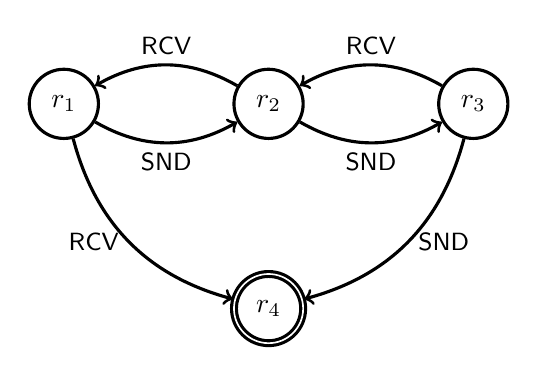
\begin{tikzpicture} [->,auto,node distance=2.6cm,line width=0.4mm]

  \node[state] (1) {$r_1$};
  \node[state] (2) [right of=1] {$r_2$};
  \node[state] (3) [right of=2] {$r_3$};
  \node[state,accepting] (4) [below of=2] {$r_4$};


  \path[every node/.style={font=\sffamily\small}]
    (1) edge [bend right] node [below] {SND} (2)
  edge [bend right] node [left] {RCV} (4)
    (2) edge [bend right] node [below] {SND} (3)
  edge [bend right] node [above] {RCV} (1)
    (3) edge [bend left] node [right] {SND} (4)
  edge [bend right] node [above] {RCV} (2); 

\end{tikzpicture}
}



\newcommand{\abpobserver}[1][]{
\begin{tikzpicture} [->,auto,node distance=2.6cm,line width=0.4mm]

%\begin{tikzpicture}[->,>=stealth',shorten >=1pt,auto,node distance=3cm,
%  thick,main node/.style={circle,fill=blue!20,draw,font=\sffamily\Large\bfseries}]

  \node[state] (1) {$o_1$};
  \node[state,accepting] (3) [right of=1] {$o_2$};
  \node[state] (2) [right of=2] {$o_3$};

  \path[every node/.style={font=\sffamily\small}]
    (1) edge [bend left] node [above] {Snd} (2)
        edge node [above] {Rcv} (3)
    (2) edge [bend left] node [below] {Rcv} (1)
        edge node [above] {Snd} (3);
\end{tikzpicture}
}

% Alter some LaTeX defaults for better treatment of figures:
    % See p.105 of "TeX Unbound" for suggested values.
    % See pp. 199-200 of Lamport's "LaTeX" book for details.
    % General parameters, for ALL pages:
    \renewcommand{\topfraction}{0.9}	% max fraction of floats at top
    \renewcommand{\bottomfraction}{0.8}	% max fraction of floats at bottom
    % Parameters for TEXT pages (not float pages):
    \setcounter{topnumber}{2}
    \setcounter{bottomnumber}{2}
    \setcounter{totalnumber}{4} % 2 may work better
    \setcounter{dbltopnumber}{2} % for 2-column pages
    \renewcommand{\dbltopfraction}{0.9}	% fit big float above 2-col. text
    \renewcommand{\textfraction}{0.07}	% allow minimal text w. figs
    % Parameters for FLOAT pages (not text pages):
    \renewcommand{\floatpagefraction}{0.7}	% require fuller float pages
% N.B.: floatpagefraction MUST be less than topfraction !!
    \renewcommand{\dblfloatpagefraction}{0.7}	% require fuller float pages

% remember to use [htp] or [htpb] for placement


\usepackage{fancyvrb}
%\DefineVerbatimEnvironment{code}{Verbatim}{fontsize=\small
%\DefineVerbatimEnvironment{example}{Verbatim}{fontsize=\small}

\usepackage{url}
\urldef{\mailsa}\path|josh0151@student.uu.se |
\urldef{\mailsb}\path|bjfo5755@student.uu.se |
\newcommand{\keywords}[1]{\par\addvspace\baselineskip
\noindent\keywordname\enspace\ignorespaces#1}


\usepackage{tikz} \usetikzlibrary{trees}
\usepackage{hyperref} % should always be the last package

% useful colours (use sparingly!):
\newcommand{\blue}[1]{{\color{blue}#1}}
\newcommand{\green}[1]{{\color{green}#1}}
\newcommand{\red}[1]{{\color{red}#1}}

% useful wrappers for algorithmic/Python notation:
\newcommand{\length}[1]{\text{len}(#1)}
\newcommand{\twodots}{\mathinner{\ldotp\ldotp}} % taken from clrscode3e.sty
\newcommand{\Oh}[1]{\mathcal{O}\left(#1\right)}

% useful (wrappers for) math symbols:
\newcommand{\Cardinality}[1]{\left\lvert#1\right\rvert}
%\newcommand{\Cardinality}[1]{\##1}
\newcommand{\Ceiling}[1]{\left\lceil#1\right\rceil}
\newcommand{\Floor}[1]{\left\lfloor#1\right\rfloor}
\newcommand{\Iff}{\Leftrightarrow}
\newcommand{\Implies}{\Rightarrow}
\newcommand{\Intersect}{\cap}
\newcommand{\Sequence}[1]{\left[#1\right]}
\newcommand{\Set}[1]{\left\{#1\right\}}
\newcommand{\SetComp}[2]{\Set{#1\SuchThat#2}}
\newcommand{\SuchThat}{\mid}
\newcommand{\Tuple}[1]{\langle#1\rangle}
\newcommand{\Union}{\cup}
\newcommand{\conf}[1]{\langle#1\rangle}
\newcommand{\subword}{\sqsubseteq}
\newcommand{\e}[1]{\emph{#1}}
\usetikzlibrary{positioning,shapes,shadows,arrows}

\usepackage{url}


\usepackage{booktabs,array}
\def\Midrule{\midrule[\heavyrulewidth]}
\newcount\rowc

\makeatletter
\def\ttabular{%
\hbox\bgroup
\let\\\cr
\valign\bgroup
\global\rowc\@ne
\hbox to 7em{\strut \hfill##\hfill}%
&&%
\global\advance\rowc\@ne
\hbox to 7em{\strut\hfill##\hfill}%
\cr}
\def\endttabular{%
\crcr\egroup\egroup}


\usepackage{amsthm}
\theoremstyle{plain}
\newtheorem{theorem}{Theorem}
\newtheorem{corollary}{Corollary}[theorem]
\newtheorem{lemma}[theorem]{Lemma}



%Specific for this document


\title{\textbf{Algorithmic Analysis of Channel machines\\ Using Small Models}}

\author{Jonathan Sharyari}
\textwidth 5.5in 
\oddsidemargin 0.5in 


\begin{document}

\maketitle


abstract
\tableofcontents
\newpage
\section{Introduction}
Todays society grows more and more dependent on computer applications\todo{Do you mean I should have a reference for this?}. Often they are used directly, for example the task of paying bills online. In other cases, applications are aiding us in a more abstract manner, e.g. controlling the elevator or planning a train schedule. The common factor between the online bank, the elevator relay and the train scheduler is that the correctness of these programs is of utter importance, where program failure could have devastating results on the economy, the infrastructure or even cause harm.

This has motivated research on various techniques to find and correct potential faults, particularly in safety-critical systems. The most common technique is that of \e{testing}, i.e. observing the system behaviour on a variety of likely or even unlikely scenarios. The widespread use of testing is well-motivated, but there are several scenarios, where testing by itself is insufficient, or difficult to carry out. It would for example be costly to verify the correctness of the aforementioned elevator only by testing, as a failure could result in damages on the system.

A technique used for verification is the process of \e{simulation}. In contrast to testing, simulation can be done in an early stage of the development. Rather than first implementing an algorithm, one may simulate an abstracted model of the algorithm which may help in ensuring its correctness or find a fault in the algorithm before development has begun. An important note is that simulation techniques are not intended to be used \e{instead} of testing, but rather in combination with testing, as an abstract model of a system can never fully represent the system as a whole.

A trend in todays computing is that applications become concurrent or distributed. Such programs are inherently difficult to verify, due to the fact that although processes themselves have finite models, the results of the behaviour of asynchronous processes may be infinite. This is the case for example when the composition of a possibly infinite number of processes is observed, a common scenario when verifying  concurrent and distributed programs. Also, we are often not interested in performing verification of a \e{specific} composition of concurrent programs, but rather in verifying that it works for \e{all} compositions.

Related to this is the necessity for distributed and concurrent programs to communicate, and to do so accurately. In general, the underlying systems that we use for our communication are inreliable, in that message loss or message corruption may occur. This happens due to a variety of reasons, may that be faults in the communication links, relays or the communicating parties themselves. To overcome this problem, communication protocols are designed to be resistent to such faults, and ensuring the correctness of these protocols is paramount when ensuring reliable communication. Even when the number of communicating processes is finite, communication protocols commonly result in infinte models, as the number of sent messages may be unbounded, and there may be an infinite number of orderings thereof. The verification of such systems, which rely on communication channels, is the focus of this thesis.

The goal of \e{model checking} is to formally verify the correctness of concurrent programs with respect  to a given specification. In general, given a model of a system and a specification of its intended properties, the task is to decide whether a model meets its specification or not.

Different representations of models and properties have been proposed, as well as techniques to perform the verification. One of the most successful and most common methods is that of \e{temporal logic model checking}. Traditionally, the model is expressed as a finite state machine and the properties as propositional logic formulae. Several verification methods for such models have been proposed\cite{mcmillan1993symbolic} and although these methods have been applied to infinite models\cite{705644}, the focus has in large been on the verification of finite models.

Another approach is taken by \cite{parosh}, in which the verification of \e{parameterized systems} is attempted. \e{Parameterized systems} are systems composed of a set of processes, where the number of processes is itself a parameter of the system. This is often the case when discussing concurrent and distributed programs. Although an undecidable problem, there are methods that can provide approximation techniques that allows us to reduce the verification task to the finite state case. These methods include \e{counter abstraction techniques}\cite{counterabstraction} and \e{invisible invariant} generation\cite{invinv}. 

In \cite{parosh}, the authors take advantage of the \e{small model property} -- if a small instance of a system is enough to exhibit the relevant behaviour of the system as a whole, that instance is a small model of the system\todo[inline]{Didn't understand the comment regarding this}. An important contribution of \cite{parosh} is that they show that this property holds for \e{quasi well-ordered systems}\cite{abdulla2010} (i.e. transitions systems monotonic with respect to a well-quasi ordering)\todo[inline]{is this good enough, or did I just explain it in a circle?}, and indicates its use for yet larger sets of systems.

Using well-known techniques of \e{abstract interpretation} combined with the idea of small models, \cite{parosh} shows that parameterized systems can in fact be reduced to finite and decidable approximations of the system, and a prototype implementation of the technique substantiates this claim by empirical results.

This essay draws the attention towards systems relying on communications over asynchronous unbounded buffers. This scenario is common in communication protocols using channels and in distributed computing\cite{fredlund2007mcerlang}. An important note is that channel systems working on \e{perfect channels} are Turing powerful\todo[inline]{Why powerful and not complete? difference?}, and therefore undecidable, but it has been shown that verification of safety properties of channel systems over \e{lossy channels}, i.e. channels that may nondeterministicly lose messages, is decidable\cite{287591}\cite{gordon}. Channels systems need not only represent communication protocols, but may also be used to described other types of programs, such as cache coherence protocols and sensor systems\cite{zuck2004}.

Inspired by \cite{parosh}, I explore the possibility of using abstract interpretation techniques and small models for systems with unbounded buffers, keeping the number of programs constant. We developed a verification technique for this purpose and the resulting model was implemented and tested. 

%As previously mentioned, this is an undecidable problem in general, and this paper does \e{not} investigate exactly what class of systems that are decidable. The experimental results show that several well-known communication protocols are indeed in the scope of the tool.

%% Is this actually a decidable problem?

\paragraph{Reading this paper} Section \ref{notation} introduces some of the terminology and notation used in this paper, whereas section \ref{definitions} contains formal definitions to some of the key concepts -- these are previously known concepts, asides from their adaption to the specific context of this thesis. Section \ref{model} introduces the concepts of small models and abstract interpretation, and relates these to buffer channels to create the theoretical model for this paper. Section \ref{extensions} introduces some extensions to this model, allowing for a wider variety of modeling scenarios. In section \ref{implementation}, some abstractions and techniques are explained that allow for an efficient implementation of the verification algorithm. Further a protocol specification language is explained, that allows a user to define and use the verification tool without knowledge of the intricacies of the internal model. The results of the verifier when applied to a number of well-known communication algorithms is presented in section \ref{results}, as well as some comparisons against the results of other verification tools.

 	

%%% Local Variables:
%%% TeX-master: "report"
%%% End:

\section{Definitions and Terms}
\subsection{Channel Systems}
We present here the basic definition of a finite-state system with unbounded channels. Such a system can be seen as to have two parts, a \e{control part} and a \e{channel part}. The channel part is a set of channels, which may be empty or contain a sequence of messages, a \e{word}. The control part is a labeled finite-state transition system\todo{Should I make labels explicit in the definition below?} The definition below is associated to systems operating on FIFO buffers, other types of systems are covered in section \ref{extensions}. 

\paragraph{Alternating Bit Protocol.} The Alternating Bit Protocol (ABP) is a distributed protocol for transmitting data from a \e{sender} to a \e{receiver} in a network. The protocol uses two unbounded channels, $ch_M$ used to transmit messages and $ch_A$ to transmit \e{acknowledgements} of received messages. The sender sends a message with sequence number x $\in$ \{0,1\} to the receiver over channel $ch_M$, who upon reception sends an acknowledgement with the same sequence number over channel $ch_A$. Both the sender and the receiver may send the same message (with the same sequence number) repeatedly. When the sender receives an acknowledgement from the receiver, the next message can be sent using the sequence number (1-x) (thus the name Alternating Bit Protocol). This is a simple protocol that operates on unbounded channels, and it is used in this paper to illustrate the theoretical concepts in a concrete setting. The behaviour of the sender and receiver process is illustrated in figure \ref{abpgraph}

\begin{figure}[h!]
\subfloat[Sender]{\label{fig:in}
\abpsender{}
}
\subfloat[Receiver]{\label{fig:in}
\abpreceiver{}
}
\caption{Program graphs of sender and receiver in the ABP protocol.}
\label{abpgraph}
\end{figure}


\paragraph{Definition}
\label{CS}
A channel system CS over a set of processes P and channels Ch is a tuple $\langle$S,$s_0$,A,C,M,$\delta$$\rangle$, where 
\begin{itemize}
\item[]
S is a finite set of control states,
\item[]
$s_0$ is an initial control state,
\item[]
A is a finite set of actions,
\item[]
Ch is a finite set of channels,
\item[]
M is a finite set of messages,
\item[]
$\delta$ is a finite set of transitions, each of which is a triple of the form $\langle s_1,op,s_2\rangle$, where $s_1$ and $s_2$ are control states, and op is a label of one of the forms

\begin{itemize}
\item
c!m, where c $\in$ Ch and m $\in$ M
\item
c?m, where c $\in$ Ch and m $\in$ M
\item
a $\in$ A.
\end{itemize}
\end{itemize}

The finite-state control part of CS is an ordinary labeled transition system with states S, initial state $s_0$ and transitions $\delta$. The channel part is represented by the set Ch of channels, which may contain a string of messages in M. The set A denotes the set of observable interactions with the environment, whereas $\delta$ may either perform an action from A, or and unobservable action, where

\begin{itemize}
\item[]
$\langle s_1, c!m, s_2\rangle$ represents a change of state from $s_1$ to $s_2$ while appending the message m to the tail of channel c
\item[]
$\langle s_1, c?m, s_2\rangle$ represents a change of state from $s_1$ to $s_2$ while removing the message m to the head of channel c
\end{itemize}

\paragraph{Example.} The alternating bit protocol can be described by a channel system CS = $\langle S,i,A,Ch,M,\delta\rangle$ such that S = {(s,r)} with \e{s} $\in$ $\{s_1,s_2,s_3,s_4\}$, \e{r} $\in$ $\{r_1,r_2,r_3,r_4\}$, \e{i} is the initial state ($s_1,r_1$), \e{A} = \{Snd, Rcv\}, \e{Ch} = \{$Ch_M,Ch_A$\}, M = \{1,0\} and delta is the set of transitions

\begin{ttabular}
$\langle s_1, Snd, s_2\rangle$ &
$\langle s_2, ch!0, s_2\rangle$ &
$\langle s_2, ch?1, s_2\rangle$ &
$\langle s_2, ch?0, s_3\rangle$ &
$\langle s_3, Snd, s_4\rangle$ &
$\langle s_4, ch!1, s_4\rangle$&
$\langle s_4, ch?0, s_4\rangle$&
$\langle s_4, ch?1, s_1\rangle$ \\

$\langle r_1, ch!1, r_1\rangle$ &
$\langle r_1, ch?1, r_1\rangle$&
$\langle r_1, ch?0, r_2\rangle$&
$\langle r_2, Rcv, r_3\rangle$&
$\langle r_3, ch!0, r_3\rangle$&
$\langle r_3, ch?0, r_3\rangle$&
$\langle r_3, ch?1, r_4\rangle$&
$\langle r_4, Rcv, r_1\rangle$
\end{ttabular}



\subsection{Channel Transition Systems}
A \e{transition system} is an abstract machine, commonly used in model checking to describe the behaviour of a system. They are in ways similar to the notion of finite state automata, with the difference that the states and transitions in a transition system need not be finite. A state of a transition system describing a program may be determined, for example, the evaluation of all variables in the program. Transitions describe how a system in a certain state can move to another state.

\paragraph{Definition}
\label{CTS}
The operational behaviour of CS is defined by the inifinite-state transition system TS = (C, $\rightarrow$) where
\begin{itemize}
\item[]
   C = (S $\times$ $\xi$) is the set of its configurations, where $\xi$ is an evaluation of the set of channels C in CS
\item[]
  $\rightarrow$ $\subseteq (S \times S)$ contains the following transitions
  \begin{itemize}
    \item
      For each observable action a $\in$ A in CS
      \[
      \dfrac{s \xrightarrow{a} s'}{(S, \xi) \rightarrow (S', \xi)}
      \]
    \item
      For each transmission action $\langle s_1, ch!m, s_2 \rangle$ in CS
      \[
      \dfrac{s \xrightarrow{ch!m} s' \wedge ch \in \xi}{(S, \xi) \rightarrow (S', \xi')} \] with \[ \xi' = \xi[ch := \xi (ch) \bullet m].
      \]
    \item
      For each reception action $\langle s_1, ch?m, s_2 \rangle$ in CS
      \[
      \dfrac{s \xrightarrow{ch?m} s' \wedge \xi(ch) = m \bullet w_1..w_n}{(S, \xi) \rightarrow (S', \xi')} \] with \[ \xi' = \xi[ch:= w_1..w_n].
      \]

  \end{itemize}
\end{itemize}

At times we may use a notation for a configuration c with explicit processes and channels, so that c = $\conf{s_1,...,s_n, ch_1,...,ch_p}$, or alternatively, with explicit processes and channel evaluations, c = $\conf{s_1,...,s_n, \xi(ch_1),...,\xi(ch_p)}$.

\paragraph{Example}
Let $c = \conf{S,\xi}$ be a configuration of the alternating bit protocol, with the channels containing the words \e{01} and \e{10} respectively. Then c may also be denoted as $c = \conf{s,r,ch_M,ch_A}$ or as $c = \conf{s_1,s_2,01,10}$. There are finitely many control states in this system, but an infinite set of channel evaluations. A transmission transition in this system is for example $\langle\conf{s_2,r_1,01,10}$, $ch_m!1$, $\conf{s_2,r_1,011,10}\rangle$. 

\subsection{Reachability and Bad Configurations}
An instance of the \e{reachability problem} is defined by a channel transition system TS = (S,$\xi$), a set of initial configurations \e{I} $\subseteq$ $S^+$ and a set \e{BAD} $\subseteq$ $S^+$ of \e{bad configurations}. We assume that \e{Bad} is the upward closure $\{c$ | $ c \in B: b \sqsubseteq c\}$ of a set of a given \e{finite} set of \e{minimal bad configurations}. \todo{Is this true in my case?}

Let c denote a configuration, then c is said to be \emph{reachable} in TS, if there are configurations $c_1...c_l$ such that $c_0$ is an initial configuration of TS and for each 0 $\leq$ i < l, $\langle c_i, c_{i+1} \rangle \in \rightarrow$.

We use $\mathcal{R}$ to denote the set of reachable states. We say that the system \e{TS} is \e{safe} if there are no reachable bad configurations, i.e. $\mathcal{R} \cap Bad$ = $\emptyset$.

\subsection{Traces}
Note that the set $\mathcal{R}$ of reachable \e{configurations} in a channel transition system is an \e{over-approximation} of the reachable \e{states} of a channel system. If $\mathcal{R} \cap Bad$ $\neq$ $\emptyset$, this does not mean that there necessarily exists a bad state in the channel system. If indeed a bad state does exist in a channel system, it is often useful not only to determine which state it is, but how that state can be reached from the initial state of the system.

Suppose $s_n$ is a bad state of a channel system \e{CS}. Then a \e{bad trace} is a sequence \e{t} = $s_0s_1...s_n$ such that for each $0 \leq i \leq (n-1)$, $\conf{s_i,r,s_{i+1}}$ $\in$ $\delta$. If \e{t} is the shortest bad trace in the system, we call it a \e{minimal bad trace}.



\section{Problem Formulation}
In \cite{parosh}, the authors propose a verification method for \e{parameterized systems} and show that how they can, under certain assumptions, be verified for an unbounded number of processes. This project is based on the results of this work, and aims to adapt this method for systems working on unbounded channels. Formally defining a model for systems working on channels, and proving that such systems have a \e{small system property} allows us to verify their correctness by only looking at finite-state representations of the system.

The goal is further to implement the proposed verification method. For such an implementation to be useful, several extensions are proposed in order to expand the context in which the system can be used. Also, a specification language is defined with which the user can easily model problems. This type of verification generally has a high demand of computational resources, thus the efficiency of the implementation is of great importance. In order to establish correctness and evaluate the efficiency of the implementation, the method is used to model several well-known communication protocols, such as the alternating bit protocol and the sliding window protocol, in order to compare its efficiency against other verification methods and establish its correctness.

\newpage
\section{Verification of Lossy Channel Systems}
\label{model}
The goal of this chapter is to formalize the use of \e{small models} for the verification of lossy channel systems, as is done in \cite{parosh}. The technique is based on the use of \e{abstract interpretation} techniques, first formalized by Cousot and Cousot\cite{cousot1977}. Abstract interpretation techniques are techniques for approximating programs. Using information about the control and data flow, i.e. the semantics of a system, an overapproximation of the possible configurations of a system can be created, which may result in an infinite set of configurations. In \cite{parosh} the authors show that such an infinite set of configurations can be safely bounded to a finite set of configurations, by finding a \e{cut-off} point for the maximum size of the evaluations.


\subsection{Views}
\label{subwords}
We define a \e{view} $v= \conf{s, \xi}$ to be a minimal representation of a set of configurations $C_v$, such that for any $c \in C_v$, $v \subword c$. Note that a view is itself a configuration, as they have the same representation, and we use the same terminology and notation for them, for example $|v|$ to denote the size. The difference is that a configuration is a single entity, whereas the view is an abstract representation of a larger set of configurations.

\paragraph{Example.} Let the view $v = \conf{(s_1, r_1), ab, cd}$, then the set $C_v$ is an infinite set, s.t. $\conf{(s_1, r_1), ab, cd} \in C_v$, $\conf{(s_1, r_1), abab, cdcd} \in C_v$ but $\conf{(s_1, r_1), ab, epsilon} \notin C_v$


\subsection{Abstraction function}
\label{alphagamma}
For a given parameter $k \in \mathbb{N}$, we use $C$ and $V$ to denote sets of configurations and views respectively, and $C_k$ and $V_k$ to denote the set of all configurations and views respectively of size up to $k$.

The abstraction function $\alpha_k: C\rightarrow 2^{V_k}$ maps a configuration $c$ into a set $V'$ of views of size up to $k$, such that for each $v\in V'$, $v \subword c$ and $size(v) \leq k$.

\paragraph{Example.} Suppose \e{c} is a configuration $\conf{s, ab,cd}$. The configuration is of size 2 and $\alpha_2(c)$ is the set


\begin{ttabular}
$\conf{s,ab,cd}$ \\
$\conf{s,a,cd}$ &
$\conf{s,b,cd}$ &
$\conf{s,\epsilon,cd}$ \\
$\conf{s,a,c}$ &
$\conf{s,b,c}$ &
$\conf{s,\epsilon,c}$ \\
$\conf{s,a,d}$ &
$\conf{s,b,d}$ &
$\conf{s,\epsilon,d}$ \\
$\conf{s,a, \epsilon}$ &
$\conf{s,b, \epsilon}$ &
$\conf{s,\epsilon,\epsilon}$ \\
\end{ttabular}
%\begin{ttabular}
%$\conf{(s),ab,cd}$ \\
%$\conf{(s),a,cd}$ &
%$\conf{(s),b,cd}$ &
%$\conf{(s),\epsilon,cd}$ \\
%$\conf{(s),a,c}$ &
%$\conf{(s),b,c}$ &
%$\conf{(s),\epsilon,c}$ \\
%$\conf{(s),a,d}$ &
%$\conf{(s),b,d}$ &
%$\conf{(s),\epsilon,d}$ \\
%$\conf{(s),a, \epsilon}$ &
%$\conf{(s),b, \epsilon}$ &
%$\conf{(s),\epsilon,\epsilon}$ \\
%\end{ttabular}


\subsection{Concretization function}
The concretization function $\gamma_k: 2^{V_k} \rightarrow 2^C$ returns, for a given set of views \e{V}, the set of configurations that can be reconstructed from the views in $V$, in other words, $\gamma_k(V) = \{c \in C$ | $\alpha_k(c) \subseteq V$\}

In general $\gamma_k(V)$ is an infinite set of configurations. We define $\gamma_k^l(V)$ := $\gamma_k(V) \cap C_l$ for some $l\geq 0$. The intuitive meaning is that $\gamma_k^l(V)$ is the set of configurations of size at most $l$ for which all views of length at most $k$ are in $V$.

\subsection{Post-Image}
For a configuration $c\in C$ of a lossy transition system $LTS = (C,\rightarrow)$, we define the \e{post-image} of \e{c} denoted $\rho(c)$ = \{$c'$ | $c \rightarrow c'$\}. Intuitively, the post-image of a configuration is the configuration obtained by firing the transitions of the transition system.

For a \e{set} of configurations $V$ we define the post-image of the set $\rho(V)$ = \{$c' | c \rightarrow c', c \in V$\}. This means that the post-image of a set $V$ of configurations is the set $\rho(V)$ containing the post-images of each configurations $c\in V$.

\subsection{Abstract Post-Image}
The \e{abstract post-image} of a set \e{V} $\subseteq$ $C_k$ is defined as $Apost_k$(\e{V}) = $\alpha_k(\rho(\gamma_k(V)))$. This means that the abstract post-image of a set $V$ is the set obtained by applying $\gamma_k$, $\rho$ and $\alpha_k$ in order to the set $V$. The procedure is illustrated in figure \ref{apost}.
\begin{figure}
\abstraction
\caption{The application order of the $\alpha$, $\rho$ and $\gamma$}
\label{apost}
\end{figure}

Note that since $V \subseteq Apost_k(V)$, $Apost_k$ is a monotonic function, thus by the Knaster-Tarski theorem, the function $Apost_k$ has a fixpoint.
%\todo[inline]{Even the infinite powerset must reach a fixpoint, right?}

\subsection{Reachability Analysis}
\label{reachcompute}
Let LTS be a lossy transition system, with an initial configuration $c^0$. Then the set of reachable configurations $\mathcal{R}$ of LTS can be computed inductively as follows: $A_0 = \{c^0\}, A_{i+1}= A_i \cup \rho(A_i)$. The finite set of configurations $\mathcal{R}_k$ with size at most $k$ can be similarly computed; $A_0$ = $\{c^0\}$, $A_{i+1} = A_i \cup (\rho(A_i) \cap C_k)$.

\subsection{Small Models}
\label{proof}
Calculating the abstract post-image of a set of views $V \subseteq C_k$ is essential for the verification procedure. As $\gamma_k(V)$ typically is infinite, this cannot be done straightforwardly. The main result of ~\cite{parosh} that it suffices to consider configurations of $\gamma_k(V)$ of sizes up to $k+1$ (i.e. $\gamma_k^{k+1}$), which is a finite set of configurations for which the abstract post-image can be computed. Formally, they show that

\begin{lemma}
\label{lemma1}
For any $k\in\mathbb{N}$, and $X\subseteq C_k$, $\alpha_k(\rho(\gamma_k(X)))$ $\cup$ $X$ = $\alpha_k(\rho(\gamma_k^{k+1}(X)))$ $\cup$ $X$.
\end{lemma}
%\todo{Why is this correct? Shouldn't it be the fixpoint of the two that is equal?}

\subsubsection{Proof of lemma 1}
We want to show that the set $\gamma_k^{k+1}(X)$ of views of size at most $k+1$ is an abstract representation of the full set $\gamma_k(X)$. In order to do this, 
%we need to show that for any reachable configuration $c$ of larger size than $k+1$, all the views of $c$ of size at most $k$ are included in the set $\gamma_k(X)$ (i.e., the configuration $c$ is abstractly represented). More precisely, 
we want to show that for any configuration $c \in$ $\rho(\gamma_k(X))$ of size $m > k + 1$ such that there is a transition  $c' \xrightarrow{r} c$, then for each view $v' \in$ $\alpha_k(c)$, the following holds: There is a configuration $d'$ $\in$ $\gamma_k^{k+1}(X)$ of size at most $k+1$ and transition $ d' \xrightarrow{r} d$ s.t. $v \in$ $\alpha_k(d)$.

Note that by design (see section \ref{LTS}), transitions only change a single evaluation, therefore, although the set of evaluations may contain multiple evaluation, we direct our focus to a single evaluation in this section.

\paragraph{Transmissions}
\label{proofTransmission}
Consider a configuration $c' = \conf{s', x} \in \gamma_k(X)$ and a transition $r: c' \xrightarrow{ch!m} c = \conf{s,x \bullet m}$. Any view $v = \conf{s', y}$ of size at most $k$ of $c$ is on one of the following forms:

\begin{enumerate}
\item
$y \subword x$, $|y| \leq k$. In this case, the set $\gamma_k^{k+1}(X)$ includes all the configurations $d'$ = $\conf{s', y}$, as $d_E' \subword c_E'$. Then $d' \xrightarrow{ch!m} d$ yields $d = \conf{s, y\bullet m}$, for which $\conf{s, y} = v$ is a view.
\item
$y = z\bullet m$ with $z \subword x$, $|z| \leq (k-1)$. The set $\gamma_k^{k+1}(X)$ includes all the configurations $d'$ = $\conf{s', z}$, as $d_E' \leq c_E'$. Then $d' \xrightarrow{ch!m} d$ yields $d = \conf{s, z\bullet m}$ which is of size at most $k$, meaning it is also a view, $d$ = $v$.
\end{enumerate}


\paragraph{Actions}
Consider a configuration $c' = \conf{s', x} \in \gamma_k(X)$ and a transition $r: c' \xrightarrow{a} c = \conf{s, x}$. Since $r$ is an action, it can be fired regardless of the channel evaluation. Therefore, if $r$ can be fired from the configuration $c'$, it may also be fired from any view $v' = \conf{s', y}$ of size at most $k$ of $c'$, resulting in a view $v =  \conf{s, y}$.

Let $\{\conf{s', w_1}, \conf{s', w_2}, \ldots,  \conf{s', w_n}\}$ be the views of $c'$, then the transition $r$ can be fired from each of these, resulting in a set $\{\conf{s, w_1}, \conf{s, w_2},\ldots \conf{s, w_n}\}$, which is the complete set of views of size at most $k$ of $c$, showing that $c$ is abstractly represented in $\gamma_k(X)$.

\paragraph{Receptions and Message Loss}
Note that receptions transitions can be seen as a special case of a message loss, where messages are lost in FIFO order, i.e. a proof of lemma 1 for message loss directly applies to the reception transitions. Consider a configuration $c' = \conf{s', x} \in \gamma_k(X)$ and a transition $r: c' \xrightarrow{*} c = \conf{s', y}$. Since $y \subword x$, the set of views $V$ of $c$ is a subset of the set of views $V'$ of $c'$.

\subsection{Verification Algorithm}
\label{verificationalgorithm}
Suppose $Bad$ is a set of bad states, such that $|b| = 0$ for all $b \in Bad$. As a result of lemma \ref{lemma1}, if $\gamma_k^{k+1}(V) \cap Bad$ = $\emptyset$ for any \e{k} $\geq$ $1$, then $\gamma_l^{l+1}(V) \cap Bad$ = $\emptyset$ for any $l \geq k$. Given a set of bad states \e{Bad}, a set of initial states \e{I} and a set of transitions, verification of a system can be done with algorithm \ref{alg1}, which was first presented in \cite{parosh}.

\begin{algorithm}
  \caption{General Verification algorithm}
  \label{alg1}
    \hspace{8pt}\textbf{for} $k := 1$ \textbf{to} $\infty$

    \hspace{16pt}\textbf{if} $\mathcal{R}_k$ $\cap$ $Bad$ $\neq$ $\emptyset$ \textbf{then return} Unsafe

    \hspace{16pt}$V := \mu X.\alpha_k(I)$ $\cup$ $Apost_k(X)$

    \hspace{16pt}\textbf{if} {$\gamma_k(V)$ $\cap$ $Bad$ = $\emptyset$} \textbf{then return} Safe
\end{algorithm}

The algorithm begins by performing a reachability analysis, as explained in \ref{reachcompute} in order to compute $\mathcal{R}_k$ and check for bad states. For any buffer size \e{k}, if a bad state is found to be reachable in $\mathcal{R}_k$, the system is unsafe and the algorithm terminates. If no such bad state was found, the algorithm continues by computing a set of configurations $X$, for which the set of concretizations $\gamma_k(X)$ is an \e{overapproximation} of reachable configurations of size $k$, reachable through configurations of size at most $k+1$ and checking for bad configurations. This is done by computing the fixpoint of $Apost_k$. If at this point no bad configuration has been found, the system can be said to be safe and the algorithm terminates. If on the other hand a bad state was found, the system is not necessarily unsafe, as \e{V} is an overapproximation of the reachable states in $\mathcal{R}_k$. The process is then repeated with a buffer size of \e{k+1}. This process is abstractly described in the flowchart in figure \ref{flow}.

\begin{figure}
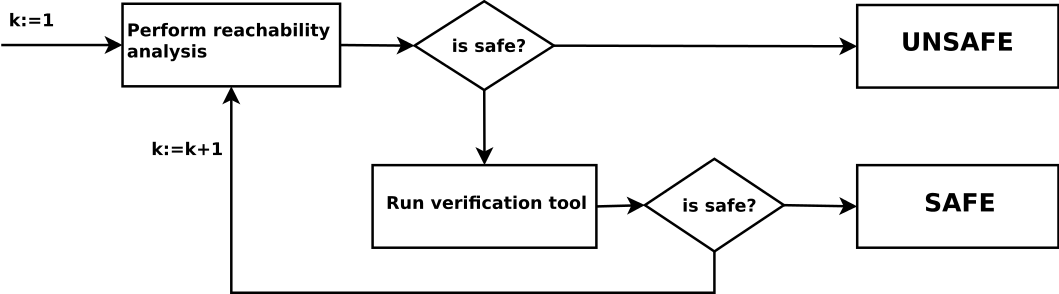
\includegraphics[width=400pt] {bilder/flowchart.png}
\caption{The general flow of the verifier.}
\label{flow}
\end{figure}

\section{Extensions}
\label{extensions}
There are several ways the channel system and the channel transition system in \ref{CS} and \ref{CTS} could be extended, in order to cope with various application scenarios. For example, we may want to model a protocol working on LIFO buffers, rather than the FIFO buffers described above. Another context may be that of a protocol communicating over an unreliable channel, introducing the possibility of \e{message loss} on the channels. In this section, we shall create models for both of these scenarios. Doing this requires us to first adapt the channel system model and the corresponding channel transition system by adding appropriate transition rules and action, and second to prove that \ref{lemma1} holds for these models.

\subsection{LIFO Channels}
\paragraph{Stack Channel System}
\label{StackCS}
In order to model a LIFO channel or a \e{stack}, we need only modify one of the transitions of the system described in \ref{CS} in such a way that transmissions and reception append and delete messages on the same end of the channels, For simplicity, we only restate this part of the channel system below. The finite-state control part of CS is an ordinary labeled transition system with states S, initial state $s_0$ and transitions $\delta$. The channel part is represented by the set Ch of channels, which may contain a string of messages in M. A set A denotes the set of observable interactions with the environment, whereas $\delta$ may either perform an action from A, or and unobservable action, where

\begin{itemize}
\item[]
$\langle s_1, c!m, s_2\rangle$ represents a change of state from $s_1$ to $s_2$ while appending the message m to the head of channel c
\item[]
$\langle s_1, c?m, s_2\rangle$ represents a change of state from $s_1$ to $s_2$ while removing the message m to the head of channel c
\end{itemize}

\paragraph{Stack Channel Transmision System}
In order to describe the transition system induced by a ChannelCS, we need only modify the transition rules of \ref{CTS} so that they reflect the changes made in \ref{StackCS}. Leaving the rest of the model unchanged, this results in $\rightarrow$ $\subseteq (S \times S)$ containing the additional transitions
\begin{itemize}
    \item
      For each observable action a $\in$ A in CS
      \[
      \dfrac{s \xrightarrow{a} s'}{(S, \xi) \rightarrow (S', \xi)}
      \]
    \item
      For each transmission action $\langle s_1, ch!m, s_2 \rangle$ in CS
      \[
      \dfrac{s \xrightarrow{ch!m} s' \wedge ch \in \xi}{(S, \xi) \rightarrow (S', \xi')} \] with \[ \xi' = \xi[ch := m \bullet \xi (ch)].
      \]
    \item
      For each reception action $\langle s_1, ch?m, s_2 \rangle$ in CS
      \[
      \dfrac{s \xrightarrow{ch?m} s' \wedge \xi(ch) = m \bullet w_1..w_n}{(S, \xi) \rightarrow (S', \xi')} \] with \[ \xi' = \xi[ch:= w_1..w_n].
      \]
  \end{itemize}

\paragraph{Proof of Lemma 1}
Only the part of the proof of lemma 1 regarding transmission rules is affected by the changes made to this system. Such a proof follows in a straightforward manner from the proof \ref{proofTransmission}, by considering configurations of the form  $\conf{S, m\bullet w'}$ rather than $\conf{S, w'\bullet m}$.

\subsection{Lossy Channels}
A lossy channel system is a system similar to \ref{CS}, with the difference that the messages on channels may be lost. In practice, data loss may appear in several contexts, e.g. data corruption, inconsistencies on weak memory models or message loss during data transmission over a network.

\paragraph{Lossy Channel Systems}
A lossy channel system is described by \ref{CS} with an additional transition $\langle s, ch*, s\rangle$ that removes a message from a channel without changing the control state.

\paragraph{Lossy Channel Transition Systems}
A lossy channel transition system TS is described by \ref{CTS} with an additional transition rule
      \[
      \dfrac{s \xrightarrow{ch*} s \wedge \xi(ch) = w_1..w_{k-1}\bullet m \bullet w_{k+1}..w_n}{(S, \xi) \rightarrow (S, \xi')} \] with \[ \xi' = \xi[ch:= w_1..w_n].
      \]

\paragraph{Proof of Lemma 1}
Trivial?  Hope so.

\subsection{Channel Systems with Synchronization}
It is not uncommon that distributed programs rely on \e{synchronization} in their program behaviour. With synchronization, we mean that two or more programs take a joint step, i.e. a transition cannot be fired unless the programs fire it together. This is particularly common in parallel programs, which may perform independent calculations but occasionally need to rendezvous. As we shall see, \ref{abpobserver}, synchronization can also be used as a modelling technique even if the program being modelled does not synchronize.

\paragraph{Channel Systems with Synchronization}
The channel system described in \ref{CS} already has the mechanisms needed in order to model synchronizing programs.\todo{Correct?}

\paragraph{Channel Transition System with Synchronization}
We modify the transition

      \[
      \dfrac{s \xrightarrow{a} s'}{(S, \xi) \rightarrow (S', \xi)}
      \]

in such a way, that an action with a label \e{l} can only be taken, if every program with that action take the action simultaneously. This corresponds to the transition

\todo{I cannot model this without talking about specific programs, which is not possible in the current definition of a channel system. I could add specific synchronization actions to that model?}


\subsection{Alternating Bit Protocol Revised}
The alternating bit protocol is a protocol designed to be resistent to message loss, therefore it is reasonable to model it using a lossy model. Furthermore, the transition system induced by the program graphs \e{abpgraph} does not provide an intuitive way to describe a set \e{Bad} of bad states. This can easily be overcome by introducing an \e{observer} program, which synchronizes with the sender and receiver.

\begin{figure}[h!]
\abpobserver
\label{abpobserver}
\end{figure}
The observer synchronizes with the sender over transitions with the label \e{Snd} and with the receiver over \e{Rcv}. If either the sender performs two transmissions (with different sequence numbers) without the receiver having received in between, or if the receiver receives two messages without the sender having transmitted in between, the observer would reach its accepting state $o_3$. This state can therefore be considered to be a minimal bad state, and any configurations describing a system with the observer in its bad state is a bad configuration.


\section{Verification method}
\label{alg1}
As a result of lemma \ref{lemma1}, if a system is found to be safe with regard to \e{Bad} for any buffer size \e{k}, it will also be safe for any buffer size larger than \e{k}. Verifying the correctness of a system can be done with the following algorithm.

\begin{algorithm}
  \caption{Verification algorithm}\label{euclid}
  \begin{algorithmic}[1]
      \For{\texttt{$r\not=0$}}
        \If {$\mathcal{R}_k$ $\cap$ $Bad$ $\neq$ $\emptyset$} 
        \State return Unsafe
        \EndIf
        \State V := $\mu X.\alpha_k(I)$ $\cup$ $Apost_k(X)$
        \If {$\gamma_k(V)$ $\cap$ $Bad$ = $\emptyset$} 
        \State return Safe     
        \EndIf
      \EndFor
\end{algorithmic}
\end{algorithm}

The algorithm has two main parts; performing a reachability analysis in order to compute $\mathcal{R}_k$ and check for bad states, and computing an overapproximation of configurations of size $k$, reachable through configurations of size at most $k+1$ and checking for bad states. For a buffer size \e{k}, If a bad state is found to be reachable in $\mathcal{R}_k$, the system is unsafe and the algorithm terminates. If no bad configuration could be reached, $Apost_k$ is applied iteratively until a fixpoint \e{V} is reached. At this point, if the set \e{V} is safe, the system can be said to be safe and the algorithm terminates. If on the other hand a bad state was found, the system is not necessarily unsafe, as \e{V} is an over-approximation of the reachable states in $\mathcal{R}_k$, the process is repeated with a buffer size of \e{k+1}.

In this rest of this section, we show how to implement this algorithm in an efficient way. We do this by beginning with a naive algorithm computing the configurations, and then step by step locating and addressing the performance issues. 

\subsection{Naive algorithm}
A naive way to generate configurations would be to perform the described operations in a way corresponding directly to the mathematical description. Here the configurations are stored in a set datastructure, thus each configuration appears at most once in the set. For each element \e{c} of the set \e{V}, the function \e{gamma}, \e{step} and \e{alpha} are performed. We assume that a set of channel symbols and a set of rules \e{R} describing the transitions are known. A rule \e{r} $\in$ \e{R} is a set of \e{predicates} - if all predicates are true for a \e{c} the rule results in a post-value \e{c'}, otherwise it results in an \e{null}-configuration.

\begin{enumerate}
\item
Gamma: For all configurations \e{c} $\in$ \e{V}, generate all configurations with channel evaluation of larger size than \e{c}. For any such configuration \e{c'}, remove those for which $alpha_k(c')$ $\not\subset$ $V$. This results the set of concretizations \e{C} of \e{c}.

\item
step: For every \e{con} $\in$ \e{C}, \e{r} $\in$ \e{R}, compute \e{r(con)}. This results in the post-image \e{post} of \e{C}.

\item
Alpha: For each element \e{p} $\in$ \e{post}, compute its views of size \e{k} and add them to \e{V'}. If \e{V'} $\cup$ \e{V} = \e{V}, a fixpoint is reached, otherwise repeat the processes with \e{V} := \e{V} $\cup$ \e{V'}.
\end{enumerate}

Although correct, this method is far from efficient. One of the main reasons is that operations are being repeated. Since if in any iteration a concretization is found, that concretization is a valid concretization in all following iterations and \e{step} and \e{alpha} will be applied again without resulting in any configurations not previously observed.

The function \e{gamma} is the heaviest of the functions. It first creates all potential concretizations of a configuration \e{c}, i.e. all combinations of channel evaluations where at least one of the channels is of a larger size than in \e{c}. Additionaly, for each of these, all their views must be computed in order to determine whether the concretization should be refuted or not.

\subsection{Less naive algorithm}
We look closer at $\gamma$, in order to address the issues mentioned above. We will show that all concretizations can be found, while considering only a subset of the potential concretizations. Furthermore, it is possible to determine whether a concretization should be refuted or not, while computing only a subset of its views. 

\paragraph{Reducing the potential concretizations.}
Given a configuration \e{c}, with channel evaluations $\xi$ such that all channels have size smaller or equal to \e{k}, a potential concretization is any configuration where at most one symbol has been added to one or more channels \e{ch} $\in$ $\xi$. As this is a large number of potential configurations, it is desireable to consider only a subset thereof, while still ensuring that all valid concretizations are eventually found. We show here that it is sufficient in each iteration to consider only the potential concretizations of \e{c}, for which only one channel has been modified, and only modifications where a symbol has been added at end (or alternatively the beginning) of a channel.

Consider a potential concretization created from \e{c}, where $n$ channels have been extended by a symbol.
If such a potential concretization is valid, any evaluation where $n'<n$ channels have been modified in a similar way will also be a valid concretization. Therefore, \e{c} will eventually be considered also when only one channel is extended in each iteration, but more iterations are required in order to find it.

Consider then a potential concretization with channel evaluation \e{e} = $w \wedge s \wedge w_1..w_l$, created by extending the channel $ww_1w_l$ with a symbol \e{m}. If \e{e} is a valid evalution, then a configuration \e{c'} must be in \e{V} such that \e{c'} has the channel evaluation $w_1 \wedge s \wedge w_1..w_{l-1}$. This channel evaluation can be extended to \e{e} by adding the symbol $w_l$ at the end of the channel.

This shows that any valid concretization will eventually be found, even if only the subset of potential concretizations are considered which are reachable by extending a single channel with a symbol at the end. This result highly reduces the number of potential concretizations inspected. If \e{s} = |$symbols$|, \e{t} is the number of channels and \e{n} = |$V$|, the naive method creates up to $n*(s^k)^t$ potential concretizations in each iteration. Using this abstraction, the number of potential concretizations is reduced to $n*s*t$.

\paragraph{Reducing the views.}
Suppose we want to determine whether \e{c} $\in$ $\gamma_k(V)$ given a configuration \e{c} and a set \e{V}. This would require that all views \e{v} $\in$ $\alpha_k(c)$ are in \e{V}. Consider a view \e{v} = $\conf{S, \xi(ch)=w}$ with size($w$) = $k$; if \e{v} $\in$ \e{V} then necessarily, any \e{v'} = $\conf{S, \xi(ch)=w'}$ with \e{w'} $\sqsubseteq$ \e{w} $\in$ \e{V}. Consequently, it is sufficient to assure that all configurations \e{c} = $\conf{S,\xi(ch_i)=w_i}$ are in \e{V}, with

\begin{itemize}
\item
size($w_i$)=$k$ if size($\xi(ch)$) $\geq$ $k$
\item
size($w_i$)= size($\xi(ch)$) if size($\xi(ch)$) < $k$.
\end{itemize}

\subparagraph{Example.} Suppose we want to determine whether \e{c} = $\conf{S, abc, def}$ is an element of $\gamma_2$. It is then sufficient to check that $\conf{S,ab,de}$, $\conf{S,ab,ef}$, $\conf{S,bc ,de}$ and $\conf{S,bc,ef}$ are in \e{V}.
\\\\\\

Using these abstraction, the computational complexity of the verifier is greatly reduced, but there are yet several ways to optimize the procedure. The bottle-neck with the procedure at its current state is the choice of a \e{Set} as lone data structure to store configurations. We expect the number of configurations to grow rather large, due to natural state-space explotion which cannot be avoided automatically (in certain cases, it could be reduced by further abstraction of the model under testing or by removing unnecessary redundancy in the model). Assuming the Set is ordered, inserting an element to the set and finding an element in the set is done in \e{O(log n)} here \e{n} is the number of elements in the set. As a consequence, onsidering the function \e{alpha}, determining whether the views of a certain configuration are in the set has complexity \e{O(plog n)} where p is the number of views of the configuration. By definition, a view (and a configuration) is of type \e{(S $\times$ $\xi$)}. For any configuration \e{c} = $\conf{s}{\xi}$, it's views will be of the type $\conf{s}{\xi'}$, i.e., all views share the same state but have different channel evaluations.

Following this reasoning, it is reasonable to divide the single \e{Set} into a Set of \e{Set}s, where each \e{Set} corresponds to a specific control-state. It is then sufficient to check for the existence of views in the \e{Set} corresponding to the control-state of the views in question.

In a best-case scenario, there would be an equal number of configurations for every state in the system. To for example check for the views of a configuration would the be reduced to \e{O(p log (n/s))} where \e{s} denotes the number of states in the system. The gains of these modifications in terms of computational complexity is difficult to determine, as the number of configurations with a certain control-state are not necessarily well-distributed, but we anticipate that the gains in many cases will be close to the best case scenario.



% Det går inte att beskriva rule-delen här, för det är mer beroende av tries.
\subsection{Even less naive algorithm}
\subsubsection{Trie}
\todo{obs!} Here there should be a description of a trie, with a reasoning about why that was chosen. It is likely that any multi-branched tree or whatever it is called would work the same. Remember to mention that hashing would have the same effect, but with this data-structure, we can guarantee to get constant time insert/search since it corresponds to a case of perfect matching.


\subsubsection{Using the Trie}
Using the above mentioned data structure, each node in the trie can be a \e{Set} with equal-state configurations, addressed by the common control-state. This leads to a speed-up both when inserting, retrieving and looking for the existence of elements in the sets, as the size of the sets will be smaller than before, when all configurations where in the same set. Retrieving and inserting nodes into the trie is done in constant time.

Having divided the configurations into equal-state groups, consider the act of firing transitions in order to create new configurations. Any configuration has a state-predicate and a channel-predicate, a state-event and a channel-event. If the predicates are fulfilled, a new configuration can be created by applying the events to the current configuration.

We show that by organizing the set of \e{rules} or transitions in a certain way in a trie, one can ensure that the state-predicate is fulfilled without specifically testing for it. A state-predicate is a predicate on the states of the processes in the system, either without any requirements on the state, or with requirements that one or more processes are in a specific state. It is therefore possible to generate a static trie of rules, addressed by control-states. Considering a transition $t_2$ with no requirements on any processes, the state-predicate will be fulfilled by any configuration, thus a corresponding rule is created in every node of the tree. Consider then a transition $t_2$ with requirements on processes all processes in the system, i.e. there is only one control-state where the transition can be taken. Such a transition corresponds to a single rule in the node addressed by that control-state. Last, consider a transition $t_3$ with requirements on a true subset of the processes in the system, then the transition can be taken from a number of control-states. These control states can be generated, and the transition will correspond to a set of rules in the nodes corresponding to those control-states.

There is a small one-time cost of creating the rule tree, but after creation, it is highly effective. It is now possible to find exactly those rules where the state-predicate is fulfilled, and there is no need to test either. This means that all computations except those where the state-predicate is fulfilled but the channel-predicate is not are actually used.

\todo{Obs, ifSeen seen? Why not ifSeen trie? Shouldn't matter?}
\todo{Shouldn't applyRules create a set instead, avoiding doubles directly?}
\paragraph{Example.} Consider the alternating bit protocol, as described in \ref{REFERERA DEN MED OBSERVER}. The system has three processes \e{Sender}, \e{Receiver} and \e{Observer} with 4, 4 and 3 states respectively. Consider then the transition with the predicates that the sender is in state 3, the observer in state 3 and they may take the synchronized transition with the action \e{Snd} to states 4 and 2 respectively. This transition has no requirements on the receiver, thus it corresponds to four rules, (3,1,3)->(4,1,2), (3,2,3)->(4,2,2), (3,3,3)->(4,3,2), (3,4,3)->(4,4,2). These rules are inserted in the nodes (3,1,3), (3,2,3), (3,3,3) and (3,4,3).

\\\\\\
The verifier at this point amounts to the following pseudo-code representation:

\todo{pseudo-code}

\subsection{Final subsection}
An efficient algorithm in this context is largely an algorithm that avoids performing unnecessary calculations, either by not creating configurations that must be discarded such as the rule-trie above or by avoiding re-calculating previously calculated results. The algorithm as described above reproduces its steps each iteration; if a configuration \e{c} can be extended to another configuration \e{c'} at any point in the verification process, then \e{c'} can and will be created in every iteration following. This includes checking whether \e{c'} is accepted or not, applying a set of rules to the configuration and adding all the views of the resulting configurations to the set. As the result of this will be exactly the same views as was considered before, the calculations are performed but the result will be duplicates and filtered out (since a \e{Set} always has unique elements}.

One way to solve this is to maintain another trie of configurations in parallell, containing exactly those configurations that have been tested and accepted. If a configuration \e{c} can be extended to \e{c'}, then we first check if \e{c'} has already been considered in a previous iteration, and if so, we discard \e{c'}. If it has not been considered, we add \e{c'} to the new trie, and perform the \e{step} and \e{alpha} steps.

Another source of repetition is the fact that there are multiple ways to create the same channel evaluations. Therefore, after a configuration has fired a set of transitions, it can result in a configuration already in the set. Instead of performing the costly calculation of finding all it's views, we first check if the newly created configuration is not in fact a duplicate by checking if it is in the new trie introduced in this section. If so, the configuration can again be discarded.

The final algorithm amounts to the following pseudo-code representation:

\subparagraph{Finding Minimal Traces}
When running the verification too, if a bad state is found we want to produce a trace leading up to the bad state. Preferably, this would be a minimal trace that leads to the bad state.
 
The proposed verification method generates a finite set of reachable states (nodes in this context), but it does not record the available transitions between the nodes (i.e. the edges). It is possible to for each node \e{n} to save all nodes \e{n} from which an edge to \e{n'} exists, and thus build the complete reachability graph of the problem. There exists efficient algorithms to solve such a problem, e.g. \e{dijkstra shortest path}, or even the shortest path between any two nodes, e.g. flow-network techniques. Although these algorithms are efficient, building the complete reachability graph would be costly in terms of memory space, as the number of edges may be much larger than the number of states.

 
We show that due to the method of iteratively constructing the graph, nodes are created in such a way, that if a node $n_{i}$ created in the \e{i}:th iteration is reached by a node $n_{i-1}$ over an edge $e_{i-1}$, the shortest path from the initial node $n_0$ will necessarily be a path $e_1...e_{i-1}$.
 
\e{Proof.} This is proven using an induction proof. We hypothesize that, if at the point of creation of $n_i$, choosing the parent node $n_{i-1}$ from which an edge $e_{i-1}$ can be taken $n_i$, the path $e_1..e_{i}$ will be the shortest path to $n_i$ and has length \e{i}. Note that the node $n_{i-1}$ must have been created in the previous iteration; had it been created earlier, the edge $e_i$ could have been taken in a previous iteration, and so $n_{i+1}$ would already be a node in the tree.
 
The base case is that for any node reachable from $n_0$ over any edge $e_0$, $e_0$ will be the shortest path and has length 1. This is trivially true.
 
Now suppose a node $n_{i+1}$ is reachable over an edge $e_i$ from a node $n_i$, and the node $n_{i+1}$ is not yet in the system. The induction hypothesis states that the path $e_1...e_i$ is the shortest path leading up to $n_i$. If $e_0..e_{i-1}e_i$ would not be the shortest path to $n_{i+1}$, there would be a path $e'_0..e'_{k-1}$ to another node $n_k$ with k < i from which $n_{i+1}$ can be reached. But any such node would have been created in the \e{k}:th iteration of the algorithm, which would contradict the fact that the node $n_{i+1}$ was not already in the system.
 
Having shown this, we need only record the information of a single parent of a node, in order to build up a tree from which the shortest path from $n_0$ to any node in the system can efficiently be found.


\swreceiver

\swobserver

\swsender


\bibliographystyle{ieeetr} 
\bibliography{references}

\end{document}
